% -*- coding: utf-8 -*-

\documentclass[a4paper,dvipdfmx]{jsarticle}
\usepackage{ascmac,alltt,txfonts,url}

\usepackage[dvipdfmx]{graphicx}
\usepackage{here}
\usepackage{fancyvrb}

\renewcommand{\ttdefault}{cmtt}
\renewcommand{\figurename}{図} 
\renewcommand{\tablename}{表} 
\DeclareMathAlphabet{\mathtt}{OT1}{cmtt}{m}{n}
\SetMathAlphabet{\mathtt}{bold}{OT1}{cmtt}{m}{n}
\setlength{\oddsidemargin}{0cm}
\setlength{\evensidemargin}{0cm}

\makeatletter

\newdimen\@mojihaba
\settowidth{\@mojihaba}{あ}

\def\tokushu#1{%
\def\tokushutitle{#1}%
\gdef\articleHeader{\hbox to\textwidth{\rule{3\@mojihaba}{1mm}%
\hbox{\small\bf\hskip1mm \tokushutitle}\leaderfill}}
}

\newdimen \JQ	\JQ .259817mm	%%%	\JQ/\Q = 10pt/9.62216pt
\newdimen \Q	\Q  .25mm	%%%	Quarter of 1mm

\def\JarticleHeader{\rule{\textwidth}{1mm}}%
\def\JarticleTitle{{\huge\bf\@title}}
\def\JarticleAuthor{\large\begin{tabular}[t]{@{}l}\@author\end{tabular}}
\newbox\@temptitlebox

\def\verse{\let\\=\@centercr 
 \list{}{\itemsep\z@ \itemindent -1.5em\listparindent \itemindent 
 \rightmargin\leftmargin\advance\leftmargin 1.5em}\item[]}
\let\endverse\endlist
\def\quotation{\list{}{\listparindent 1.5em
 \itemindent\listparindent
 \rightmargin\leftmargin \parsep 0pt plus 1pt}\item[]}
\let\endquotation=\endlist
\def\quote{\list{}{\rightmargin\leftmargin}\item[]}
\let\endquote=\endlist
\def\abstquotation{\list{}{\listparindent 1.5em
 \itemindent\listparindent
 \leftmargin 5mm
 \rightmargin\leftmargin \parsep 0pt plus 1pt}\item[]}
\let\endabstquotation=\endlist
\def\quote{\list{}{\rightmargin\leftmargin}\item[]}
\let\endquote=\endlist

\global\def\@maketitle{\newpage \null
\hbox{\vbox to193.5\Q{\baselineskip=10mm % 193.5\Q = 9*\baselineskip
\begin{flushleft}
\JarticleHeader
% following extra vskip together with baselineskip(10mm) will produce
% appropriate 10mm/6mm gap between the rule and title
% This assumes that title is typeset with 28Q(7mm) font, and baseline
% is set 1mm above the bottom of the font.
\setbox\@temptitlebox\hbox{JarticleTitle}\ifdim\wd\@temptitlebox>\textwidth\vskip2mm\else\vskip6mm\fi
\leftskip=5mm
\JarticleTitle
\vskip6mm % to leave 10mm gap between title and author
\JarticleAuthor
\end{flushleft}\vfil}}
%\JEabstInsert
  \begin{small}
    \begin{abstquotation}
      \Jabstcontent
    \end{abstquotation}
  \end{small}
}

\long\def\Jabstract#1{\global\long\def\Jabstcontent{\noindent\ignorespaces #1}}
\def\Jabstcontent{\relax}

\makeatother

\usepackage{fancyhdr}
\pagestyle{fancy}
\lhead{VHDL/Verilog HDL 入門}
\rhead{}
\rhead{\thepage{}}
\cfoot{}
\renewcommand{\headrulewidth}{0.5pt}
\pagestyle{fancy}

\Jabstract{%
\\
代表的なハードウェア記述言語VHDLとVerilog HDLの基礎概念と文法を学ぼう
}

\begin{document}

\title{VHDL/Verilog HDL 入門}
\author{}
\date{2019年 8月22日~~第3.1版}
\maketitle

\section{はじめに}

本章では,ハードウェア記述言語(HDL; Hardware Description Language)のうち,よく使用されるVHDLとVerilog HDLの二つのHDLの基本文法を説明します.ちょっとした違いを発見しながら読み進めると面白いでしょう.

ソフトウェア・プログラミングで使用するCやJava,コミュニケーションで使用する英語についても,正しく使用するために文法の知識は欠かせません.同じようにHDLで設計する際も文法の知識が必要です.ここで,基本文法をしっかり押さえましょう.

\section{ハードウェア記述言語の基本概念}

プログラミング言語に多くの種類があるように,ハードウェア記述言語(HDL)にもさまざまな種類があります.その中でもよく利用されるのが,VHDLとVerilog HDLです.VHDLとVerilog HDLは,どちらも,ハードウェアを表現するための似たような概念を取り扱うことができる言語です.

ただし,似たような概念でもそれぞれの言語で使用する言葉が違うので注意が必要です.両方の言語に共通する概念と,言語の特徴について説明します.

\subsection{構造の基本 --- エンティティ/モジュール}

どの言語にも基本的な構造があります.たとえば,Cでは関数,Javaではクラスなどです.HDLでは,与えられた入力に対して出力を生成するブロックが基本的な単位です(図\ref{fig:design_unit}).このブロックをVHDLではエンティティ(\verb|entityt|),Verilog HDLではモジュール(\verb|module|)と呼びます.ただし,この章では,特にVHDLやVerilog HDLに違いがない説明では,モジュールと呼ぶことにします.

 \begin{figure}[H]
  \begin{center}
   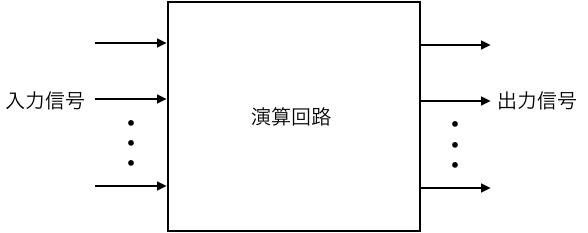
\includegraphics[width=.5\textwidth]{chapter02_figures/design_unit.png}
  \end{center}
  \caption{ハードウェア・プログラミングの基本的な単位 \label{fig:design_unit}}
 \end{figure}

通常のプログラミング言語とHDLの大きな違いは,エンティティ/モジュールは,最初から最後まで与えられた入力に対する出力を生成し続けるということです.Cなどで関数を呼び出す場合,mainプログラムからその関数内へ処理が移ります(\ref{fig:software_running_model}).処理を終えると戻り値を呼び出し元に返し,mainプログラムが再び動き始めます.つまり,mainプログラムは,呼び出した関数の処理が完了するまで待たされます.これは,プログラム・カウンタが,プログラムを順々に呼び出して実行するからです.

 \begin{figure}[H]
  \begin{center}
   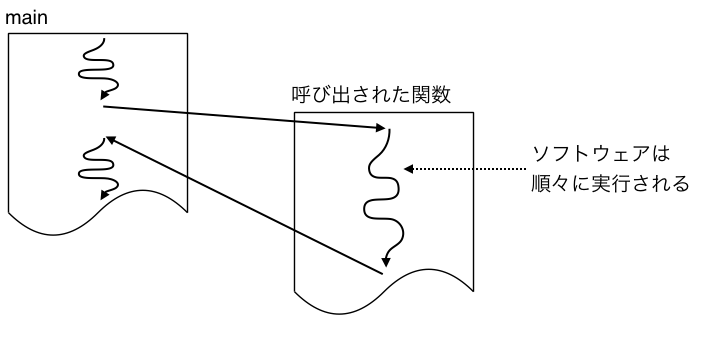
\includegraphics[width=.75\textwidth]{chapter02_figures/software_running_model.png}
  \end{center}
  \caption{Cで記述した一般的なソフトウェア・プログラムの実行の様子 \label{fig:software_running_model}}
 \end{figure}

一方,HDLで記述されたエンティティ/モジュールには,共通のプログラム・カウンタのような,複数の演算回路の動作を制御する仕組みはありません.(図\ref{fig:hardware_instances}).どのモジュールも常に存在し,独立して動作します.したがって,特定の入力を与えると出力を返すというよりも,入力されているデータに対して出力するデータを作り続けているというイメージになります.複数のモジュール間で制御が必要であれば自分で,そのように設計する必要があります.

 \begin{figure}[H]
  \begin{center}
   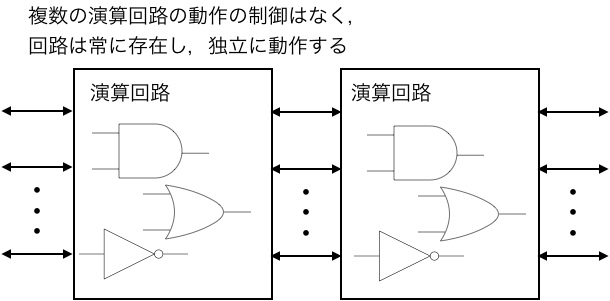
\includegraphics[width=.65\textwidth]{chapter02_figures/hardware_instances.png}
  \end{center}
  \caption{ハードウェアは常に存在し,演算回路の動作が制御されることはない(制御が必要なら自分で記述する必要がある) \label{fig:hardware_instances}}
 \end{figure}

\subsection{2種類の基本処理方法 --- 同時処理文と順次処理文}
繰り返しになりますが,ハードウェア・プログラミングでは,独立して動作するモジュールを扱う必要があります.すなわちハードウェアを記述するための言語では,独立して動作する同時並行的な処理を記述できる必要があります.とはいえ,実現したい処理によっては,条件分岐のような依存関係のある処理の記述が望まれます.これらの要求を満たすため,VHDLとVerilog HDLのどちらも,同時処理文と順次処理文と呼ばれる二種類の記述方式をサポートしています.具体的な記述方法は後で説明しますが,それぞれの考え方を頭に入れておいてください.

\paragraph{同時処理文}
同時処理文とは,周りの処理に依存せず独立して動作する処理です.複数の同時処理文は,ある特定の時点で一斉に処理されます.そのため,記述順や各処理文の間には,構文的な順序が存在せず,「ある時点」で入力された値に従って出力が生成されます.出力が確定するまでの時間は,物理的にデバイスの中を電気が流れる速さや信号遅延に依存します.

\paragraph{順次処理文}
順次処理文は,複数の処理同士に構文などによって順序が規定された処理です.たとえば,ソフトウェアには欠かせない分岐などの制御文の表現には順序が必要になります.

\subsection{使用できる変数 --- 数値と信号}
プログラミング言語と同じようにHDLでも変数を利用できます.VHDLでもVerilog HDLでも,変数はすべて型を持ちます.ハードウェアとして,基本的な型は1本の信号線です.また,信号線を束ねた配列もサポートされます.このほかに,整数や自分で定義した型も利用できます.

変数は,英数字からなる名前を付けることができます.変数名の先頭は英字または「\_」で始める必要があり,末尾を「\_」にしてはいけません.Verilog HDLでは,大文字と小文字は区別されます.

\subsection{演算の基本 --- 算術/論理減算,比較,代入}
VHDLおよびVerilog HDLでは加減算や論理演算,比較などの演算子を利用することができます.ソフトウェア・プログラミングの場合は演算子を使って記述された処理はプロセッサに与える命令に変換されますが,HDLの場合は,その演算に相当するハードウェア・ロジックとしてLUTやFFなどの組み合わせに合成されます.FPGAの中には,小さなディジタルシグナルプロセッサや乗算器を持つものがあり,条件にうまく合致すると,それらが使用されます.

HDLでもソフトウェア・プログラミング同様に,演算した結果を代入演算を利用して,ほかの(あるいは同じ)変数に代入することができます.HDLの代入には,ブロッキング代入とノンブロッキング代入の2種類があります.ブロッキング代入は,その時点で値を代入して次に進む代入です.一方,ノンブロッキング代入は,複数の代入文において,それらの代入の同時実行を規定します.Cなどで記述した単一スレッドのソフトウェア・プログラムの代入は,HDLでいうところのブロッキング代入に相当します.

\subsection{値の基本 --- '0','1','Z','X'}
ハードウェアの値は'0'と'1'の値をとります.加えて,ハードウェアにはハイ・インピーダンスという,「抵抗が無限大」を意味する状態が存在します.VHDLやVerilog HDLでは'Z'で表されます.値として「抵抗が無限大」というのは,少しわかりにくいかもしれません.物理的には,図\ref{fig:high_imp_image}のようにスイッチを切った状態をイメージしてください.複数の信号が一つにまとめられるとき,'Z'は,「ほかの値に影響を与えない」ということを意味します.

 \begin{figure}[H]
  \begin{center}
   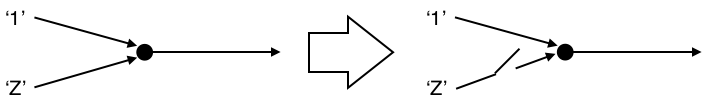
\includegraphics[width=.65\textwidth]{chapter02_figures/high_imp_image.png}
  \end{center}
  \caption{HDLではハイ・インピーダンスでスイッチオフを記述できる \label{fig:high_imp_image}}
 \end{figure}

また,'0'でも'1'のどちらでもいい値として不定値という概念があります.これは,'X'と表現されます.

ソフトウェア・プログラミングでは,通常,'0'と'1'の2値をとる値をビットと呼びますが,'Z'と'X'も加えた4つの値をとる信号が便宜上ビットと呼ばれることが多くあります.

\subsection{文末には「;」を付ける}
VHDLもVerilog HDLも,演算処理や変数定義などの文の終わりには「;」(セミコロン)を付けます.ただし,両言語ともソフトウェアのプログラミング言語では少し首をかしげてしまうような,「;」を付けないケースが存在するので注意が必要です.

\section{VHDLの基本文法のルール}

VHDLの基本的な文法を説明します.

\subsection{コメント}
多くのソフトウェア・プログラミング言語と同様に,VHDLでもソースコード中にコメントを書くことができます.VHDLでは,「\verb|--|」から行末までがコメントになります.

\subsection{モジュールの構成}
図\ref{fig:vhdl_module_overview}に,VHDLで記述するモジュールの概要を示します.VHDLでは,対象とするモジュールを大きく\verb|entity|と\verb|architecture|に分けて記述します.\verb|entity|には外部に接続される入出力ポートの宣言などの回路の外枠を,\verb|architecture|には使用する関数の定義や処理内容など,回路の内部を定義します.

 \begin{figure}[H]
  \begin{center}
   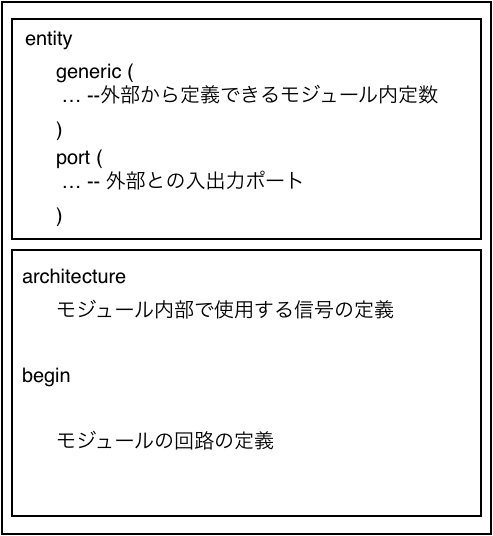
\includegraphics[width=.4\textwidth]{chapter02_figures/vhdl_module_overview.png}
  \end{center}
  \caption{VHDLのモジュール定義はentityとarchitectureから構成される \label{fig:vhdl_module_overview}}
 \end{figure}

\subsection{即値の表現方法}
VHDLでは,ソース・コードの中に定数の値を記述できます(表1).複数の信号線を束ねた値は,信号線の本数分だけ各信号に相当する値を並べて表現します(たとえば4bitなら\verb|"0000"|など).また,「\verb|X"01"|」と記述することで16進数で数を表記できます.よく用いられる代表的な定数表現には,表\ref{tbl:vhdl_constants}のようなものがあります.

\begin{table}[H]
\begin{center}
 \begin{tabular}{l|l}
 \hline
  説明                       & 値の例 \\\hline\hline
  1本の信号線がとる信号の値  & \verb|'1'|,\verb|'0'| ,\verb|'Z'|,\verb|'X'|  \\\hline
  複数の信号線がとる信号の値 & \verb|"111"|,\verb|"0100"| ,\verb|X"10"| \\\hline
  整数                       & \verb|32|,\verb|8| ,\verb|1000| \\\hline
  真偽値                     & \verb|true|,\verb|false|\\\hline
 \end{tabular}
\end{center}
\caption{VHDLで記述できる定数の例\label{tbl:vhdl_constants}}
\end{table}


\subsection{型}
VHDLの変数はすべて型を持ちます.たくさんの型が定義されており,また,独自の型も定義できます.よく使用される5つの型を表\ref{tbl:vhdl_types}に示します.基本的には,\verb|std_logic|,\verb|std_logic_vector|はハードウェアの信号に相当する型,\verb|signed|や\verb|unsigned|は加減算などの算術演算ができる値を表現するために用いる型,一般的な数値を表現できる\verb|integer|です.

\begin{table}[H]
\begin{center}
 \begin{tabular}{l|l}
 \hline
  型名                                  & 説明 \\\hline\hline
  \verb|std_logic|                      & 1bitの信号線     \\\hline
  \verb|std_logic_vector(n-1 downto 0)| & n-bitの信号線    \\\hline
  \verb|unsigned(n-1 downto 0)|         & n-bitの符号なしの算術演算可能な値 \\\hline
  \verb|signed(n-1 downto 0)|           & n-bitの符号ありの算術演算可能な値 \\\hline
  \verb|integer n to m|                 & nからmまでの整数 \\\hline
 \end{tabular}
\end{center}
\caption{VHDLで用いられる型の例\label{tbl:vhdl_types}}
\end{table}

\subsubsection{1-bitの信号}
\verb|std_logic|は,VHDLの基本となる1bitの信号に相当する型です.'0','1'のほかに,ハイ・インピーダンスを示す'Z',不定値を示す'X'を値としてとれます.これらの値は,ハードウェアにそのまま対応します.

\subsubsection{n-bitの信号}
\verb|std_logic_vector(n downto 0)|は,\verb|std_logic|がn個並んだn-bitの信号線に相当する型です.「n-bitの\verb|std_logi_vector|型」と呼びます.\verb|std_logic_vector|型の変数aの中の要素を,a(3),a(4 downto 2)などとして取り出せます.前者は\verb|std_logic|型,後者は3bitの\verb|std_logic_vector|型です.「\verb|downto|」は\verb|std_logic|の並びに,MSBから降順で番号を付けることを意味します.つまり,\verb|std_logic_vector(n-1 downto 0)|のビット列の場合,MSBが\verb|std_logic_vector(n-1)|で,LSBが\verb|std_logic_vector(0)|です.\verb|to|を使うことで逆順に並べることもできます.その場合は,\verb|std_logic_vector(n upto 0)|のように書きます.

\subsection{モジュールの外枠の記述 --- entity}
\verb|entity|は,モジュールの外枠に相当し,モジュールの名前と入出力の信号で定義されます.たとえば,
次の記述は,入力信号にpClkとpReset,出力信号にQを持つtestという名前のモジュールの外枠の定義に相当します.

\begin{figure}[H]
\begin{quote}
\begin{Verbatim}[frame=single, numbers=left, baselinestretch=0.8]
entity test is
 port (
   pClk   : in std_logic;
   Q      : out std_logic;
   pReset : in std_logic -- 最後の一つの後には";"をつけない
 );
end entity;
\end{Verbatim}
\end{quote}
\end{figure}

\subsubsection{ポートを定義する}
ポートは,ハードウェア・モジュールの入出力です.\verb|entity|の中の\verb|port( 〜 );|の中に信号を方向と型を指定して定義します.信号の方向には\verb|in|(入力)と\verb|out|(出力),\verb|inout|(入出力)の3種類があります.各ポートは「名前 : 方向 型」で定義されます.たとえば,
\begin{figure}[H]
\begin{quote}
\begin{Verbatim}[frame=single, numbers=left, baselinestretch=0.8]
pClk : in std_logic
\end{Verbatim}
\end{quote}
\end{figure}
という記述は,\verb|pClk|という名前の型が\verb|std_logic|の入力ポート(\verb|in|)の定義に相当します.同じ方向,型の複数のポート名は「,」で並べて定義することもできます.たとえば,
\begin{figure}[H]
\begin{quote}
\begin{Verbatim}[frame=single, numbers=left, baselinestretch=0.8]
pR, pG, pB : in std_logic
\end{Verbatim}
\end{quote}
\end{figure}
として,3つの入力信号\verb|pR|,\verb|pG|,\verb|pB|をまとめて定義できます.

\subsubsection{定数を定義する}
\verb|entity|の中にモジュールの中で使用する定数を定義できます.
\begin{figure}[H]
\begin{quote}
\begin{Verbatim}[frame=single, numbers=left, baselinestretch=0.8]
entity test is
  generic (
    width  : integer := 640;
    height : integer := 480
  );
  port (
    pClk : in std_logic;
    Q : out std_logic;
    pReset : in std_logic
  );
end test;
\end{Verbatim}
\end{quote}
\end{figure}
ここでは,\verb|width|という名前で値が640の\verb|integer|型,すなわち整数の定数を定義しています.この定数は\verb|entity|内部,および内部処理を記述する\verb|architecture|の中で使用できます.

\subsection{内部処理の記述 --- architecture}
VHDLでは,\verb|architecture|にモジュールの処理内容を記述します.記述の基本的な流れは次の通りです.
\begin{figure}[H]
\begin{quote}
\begin{Verbatim}[frame=single, numbers=left, baselinestretch=0.8]
architecture RTL of test is
  (ここに変数の定義などを書く)
begin
  (ここに処理内容を記述する)
end RTL;
\end{Verbatim}
\end{quote}
\end{figure}
上記は,\verb|test|という名前のモジュールの中身を記述するためのブロックです.

\subsection{変数の定義}
\verb|architecture|内部で使用する変数として,変数を\verb|signal|というキーワードを使って定義できます.初期値は省略可能です.
\begin{figure}[H]
\begin{quote}
\begin{Verbatim}[frame=single, numbers=left, baselinestretch=0.8]
signal 名前 : 型 := 初期値;
\end{Verbatim}
\end{quote}
\end{figure}

たとえば,10ビットの配列は下記のように定義します.
\begin{figure}[H]
\begin{quote}
\begin{Verbatim}[frame=single, numbers=left, baselinestretch=0.8]
signal counter : std_logic_vector(9 downto 0);
\end{Verbatim}
\end{quote}
\end{figure}

また,\verb|generic|で定義した値である\verb|width|を使用して,幅widthの\verb|std_logic_vector|型の信号を次のように定義できます.ここで「\verb|width−1|」の値は合成時に決定されます.
\begin{figure}[H]
\begin{quote}
\begin{Verbatim}[frame=single, numbers=left, baselinestretch=0.8]
signal counter : std_logic_vector(width-1 downto 0);
\end{Verbatim}
\end{quote}
\end{figure}

\subsection{演算子と演算}
代表的な演算子を表\ref{tbl:vhdl_operator}にまとめます.論理演算子を\verb|std_logic_vector|型に定義した場合は,対応する各ビットの値同士に論理演算を適用した結果を返します.たとえば,「\verb|"10" and "11"|」は「\verb|"10"|」になり,「\verb|"10" or "11"|」は「\verb|"11"|」になります.比較演算の結果は,\verb|true|か\verb|false|の真偽値になります.よくあるプログラミング言語に備わっている演算が備わっていることがわかります.ただし,表\ref{tbl:vhdl_operator}の説明に(*1)をつけている,算術演算や数値の大小を比較する演算では\verb|unsigned|型,\verb|signed|型あるいは\verb|integer|の変数や定数,あるいは数値に相当する即値にしか利用できません.

\begin{table}[H]
\begin{center}
 \begin{tabular}{l|l|l}
 \hline
  種類      & 演算子         & 説明 \\\hline\hline
  論理演算  & \verb|a and b| & 論理積.aとbが\verb|'1'|なら\verb|'1'|.さもなければ\verb|'0'|.\\\cline{2-3}
            & \verb|a or b|  & 論理和.aとbのどちらか又は両方が\verb|'1'|なら\verb|'1'|.さもなければ\verb|'0'|.\\\cline{2-3}
            & \verb|a xor b| & 排他的論理積.aとbの一方だけが\verb|'1'|なら\verb|'1'|.さもなければ\verb|'0'|.\\\cline{2-3}
            & \verb|not a|   & 否定.aが\verb|'0'|なら\verb|'1'|.\verb|'1'|ならverb|'0'|\\\hline
  比較演算  & \verb|a = b|   & aとbが等しい場合\verb|true|.さもなければ\verb|false|\\\cline{2-3}
            & \verb|a /= b|  & aとbが等しくなければ場合\verb|true|.さもなければ\verb|false|\\\cline{2-3}
            & \verb|a > b|   & aがbがより大きいなら\verb|true|.さもなければ\verb|false|.(*1)\\\cline{2-3}
            & \verb|a < b|   & aとbがより小さいなら\verb|true|.さもなければ\verb|false|.(*1)\\\cline{2-3}
            & \verb|a >= b|  & aとb以上なら\verb|true|.さもなければ\verb|false|.(*1)\\\cline{2-3}
            & \verb|a <= b|  & aとb以下なら\verb|true|.さもなければ\verb|false|.(*1)\\\hline
  算術演算  & \verb|a + b|   & aとbの足し算 (*1)\\\cline{2-3}
            & \verb|a - b|   & aとbの引き算 (*1)\\\cline{2-3}
            & \verb|a * b|   & aとbの引き算 (*1)\\\cline{2-3}
            & \verb|a / b|   & aとbの割り算 (*1)\\\cline{2-3}
            & \verb|a ** b|  & aのb乗 (*1)\\\hline
   配列操作 & \verb|a & b|   & aとbをこの順に並べた信号線の束を作る \\\cline{2-3}
            & \verb|a(b) |   & aのb番目の信号を取り出す \\\cline{2-3}
            & \verb|a(b downto c) | & aのb番目からc番目の信号線の束を取り出す \\\hline
 \end{tabular}
\end{center}
\caption{VHDLで用いられる演算の例\label{tbl:vhdl_operator}}
\end{table}

\subsubsection{演算結果の代入}
演算の結果は代入文でほかの(あるいは同じ)変数へ代入できます.代入にはブロッキング代入とノンブロッキング代入があります.
\begin{figure}[H]
\begin{quote}
\begin{Verbatim}[frame=single, numbers=left, baselinestretch=0.8]
:= ブロッキング代入
<= ノンブロッキング代入
\end{Verbatim}
\end{quote}
\end{figure}
たとえば,
\begin{figure}[H]
\begin{quote}
\begin{Verbatim}[frame=single, numbers=left, baselinestretch=0.8]
Q <= counter(width-1);
\end{Verbatim}
\end{quote}
\end{figure}
という記述は,\verb|std_logic_vector|型の変数\verb|counter|の\verb|(width-1)|番目を取り出し,\verb|Q|に代入するハードウェアの記述に相当します.VHDLでは,\verb|signal|変数には,初期化時以外でブロッキング代入を使用することはできません.

\subsubsection{型の変換}
VHDLは型の制約が強い言語で.代入は同じ型の変数同士でしか認められません.また演算子も適用可能な型があらかじめ決められています.そのため,幅の違う\verb|std_logic_vector|同士で値を定義する場合には,ビット幅を削る/足すなどして同じ幅にしなければいけません.たとえば,aとbが,それぞれ幅16-bit,8-bitの\verb|std_logic_vector|型であれば,
\begin{figure}[H]
\begin{quote}
\begin{Verbatim}[frame=single, numbers=left, baselinestretch=0.8]
a <= "00000000" & b; -- 足りない8bitを8bitの0(="00000000")で埋めている
b <= a(7 downto 0); -- aの下位8bitだけをbに代入している
\end{Verbatim}
\end{quote}
\end{figure}
などとする必要があります.

型の変換には専用の関数を利用します.たとえば,\verb|std_logic_vector|を\verb|unsigned|型あるいは\verb|signed|型に変換するためには,それぞれ\verb|unsigned|関数あるいは\verb|signed|を用います.
\begin{figure}[H]
\begin{quote}
\begin{Verbatim}[frame=single, numbers=left, baselinestretch=0.8]
unsigned(c);
\end{Verbatim}
\end{quote}
\end{figure}
と記述すると\verb|std_logic_vector|型の変数\verb|c|を\verb|unsigned|型に変換できます.

逆に,\verb|unsigned|型や\verb|singed|型の変数を\verb|std_logic_vector|型に変換する場合には,\verb|std_logic_vector|関数を用います.
\begin{figure}[H]
\begin{quote}
\begin{Verbatim}[frame=single, numbers=left, baselinestretch=0.8]
std_logic_vector(d);
\end{Verbatim}
\end{quote}
\end{figure}
と記述すると\verb|unsigned|型の変数\verb|d|を\verb|std_logic_vector|型に変換できます.

\verb|integer|型の変数を\verb|unsigned|型や\verb|signed|型に変換する場合には,\verb|to_unsigned|あるいは\verb|to_signed|を使います.たとえば,\verb|integer|型の変数\verb|k|をn-bitの\verb|unsigned|型に変換する場合は,2番目の引数にビット数\verb|n|を指定して,
\begin{figure}[H]
\begin{quote}
\begin{Verbatim}[frame=single, numbers=left, baselinestretch=0.8]
to_unsigned(k, n);
\end{Verbatim}
\end{quote}
\end{figure}
と記述します.

一般に,VHDLでは,\verb|std_logic_vector|型の変数に対して算術演算は記述できません.そのため,\verb|std_logic_vector|と定数の加減算や比較演算する場合には,一度\verb|unsigned|型に変換して演算する必要があります.たとえば,幅nの\verb|std_logic_vector|の変数counterに定数\verb|1|を加算する場合には,次のように,一度\verb|unsigned|型に変換して演算した後で\verb|std_logic_vector|型に戻す必要があります.
\begin{figure}[H]
\begin{quote}
\begin{Verbatim}[frame=single, numbers=left, baselinestretch=0.8]
counter <= std_logic_vector(unsigned(counter) + 1);
\end{Verbatim}
\end{quote}
\end{figure}

\subsubsection{シフト演算}
VHDLには,ソフトウェア・プログラミング言語で一般的なシフト演算子に相当する演算子がありません.VHDLでは配列操作の演算を用いて似たような操作ができます.たとえば,幅n-bitの\verb|std_logic_vector|型の変数counterを右に1つシフトしたい場合には,次のように記述します.
\begin{figure}[H]
\begin{quote}
\begin{Verbatim}[frame=single, numbers=left, baselinestretch=0.8]
counter <= '0' & counter(n-1 downto 1);
\end{Verbatim}
\end{quote}
\end{figure}
左に2つシフトしたい場合には,
\begin{figure}[H]
\begin{quote}
\begin{Verbatim}[frame=single, numbers=left, baselinestretch=0.8]
counter <= counter(n-3 downto 0) & "00";
\end{Verbatim}
\end{quote}
\end{figure}
となります.

\subsection{同時処理文}
VHDLでは単に並べて記述された文は,同時処理文として解釈されます.
それらは合成ツールにより並列に解析され,回路に合成されます.すなわち,記述された内容はその順序に依存しません.
たとえば,
\begin{figure}[H]
\begin{quote}
\begin{Verbatim}[frame=single, numbers=left, baselinestretch=0.8]
c <= a and b;
e <= c and d;
\end{Verbatim}
\end{quote}
\end{figure}
と書いても,
\begin{figure}[H]
\begin{quote}
\begin{Verbatim}[frame=single, numbers=left, baselinestretch=0.8]
e <= c and d;
c <= a and b;
\end{Verbatim}
\end{quote}
\end{figure}
と書いても,同じように図\ref{fig:parallel_vhdl}の回路が合成されます.

 \begin{figure}[H]
  \begin{center}
   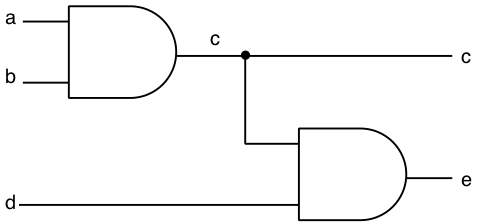
\includegraphics[width=.4\textwidth]{chapter02_figures/parallel_vhdl.png}
  \end{center}
  \caption{同時処理文は,記述順によらず解析・合成される \label{fig:parallel_vhdl}}
 \end{figure}


\subsection{順次処理文 --- process文}
順次処理文では記述された順序に従って意味が解析され,回路が合成されます.そのため,複雑な制御構文を使用できます.VHDLでは,\verb|architecture|中で\verb|process|を使って順次処理文を記述するためのブロックを作ることができます.\verb|process|文の基本的な構文を次に示します.
\begin{figure}[H]
\begin{quote}
\begin{Verbatim}[frame=single, numbers=left, baselinestretch=0.8]
process(a, b)
begin
  c <= a and b;
  d <= a or b;
end process;
\end{Verbatim}
\end{quote}
\end{figure}

ここで,\verb|process()|の「\verb|()|」内の変数のリストをセンシティビティ・リストといいます.このリストに列挙した変数の信号が変化すると\verb|process|の中の回路が動作し出力値が変更されます.ノンブロッキング代入は,process内の記述が順に解釈された後で,同時に信号が確定します.このprocess文は,図\ref{fig:process_example}のような回路を生成します.あくまで文が順に解釈されるだけで,順に処理される回路が生成できるわけではない,ことに注意する必要があります.

 \begin{figure}[H]
  \begin{center}
   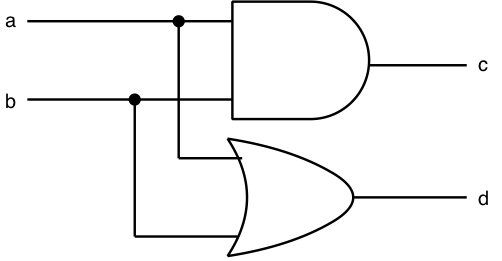
\includegraphics[width=.4\textwidth]{chapter02_figures/process_example.png}
  \end{center}
  \caption{順次処理文中の複数のノンブロッキング文は順に解釈され,最後に値が同時に確定する \label{fig:process_example}}
 \end{figure}

\verb|process|文の中にでてくる入力変数(式の右辺にでてくる変数)がすべてセンシティビティ・リストに列挙されている場合,入力が変化する度に回路が動作し,出力変数(式の左辺)の値が変更されます.つまり,その\verb|process|文から生成される回路では,何も状態を保存する必要がありません.そのため,図\ref{fig:process_example}のような記憶素子を必要としない組み合わせ回路として構成されます.

センシティビティ・リストにない変数が右辺に使われる.次のようなprocess文を考えてみます.
\begin{figure}[H]
\begin{quote}
\begin{Verbatim}[frame=single, numbers=left, baselinestretch=0.8]
process(a)
begin
  c <= a and b;
  d <= a or b;
end process;
\end{Verbatim}
\end{quote}
\end{figure}
ここでは,センシティビティ・リストに「b」がなく,入力変数が全部列挙されていません.この回路では,bの値が変化しても出力先であるcとdの値は変化しません.つまり,図\ref{fig:process_example}のように,入力であるaとbを出力のcとdに直接接続することができず,cとdの値を保存する機構,記憶素子が必要となり,組み合わせ回路として合成されません.「同じように記述したつもりでも違う回路になるかもしれない」ということを覚えておいてください.

VHDLの\verb|process|文では,ブロッキング代入可能な\verb|variable|変数を利用できます.\verb|variable|変数は,順次処理文において便宜的に一時的な値を格納しておくためのものです.長く複雑な演算を行う場合に,ソース・コードの見通しをよくできます.
たとえば,次のように使います.
\begin{figure}[H]
\begin{quote}
\begin{Verbatim}[frame=single, numbers=left, baselinestretch=0.8]
process(a,b)
  variable tmp0 : std_logic;
  variable tmp1 : std_logic;
begin
  tmp0 := a and b;
  tmp1 := a or b;
  c <= tmp0 xor tmp1;
end process;
\end{Verbatim}
\end{quote}
\end{figure}
ここでは,tmp0とtmp1がvariable変数です.ブロッキング代入における演算の結果がそれぞれ代入されています.ブロッキング代入のため,合成ツールがこの構文に出会ったところで,tmp0の値は(a and b)に,tmp1の値は(a or b)にすぐさま置き換わります.つまり,これは,\verb|c <= (a and b) xor (a or b)|という回路として合成されます.

\subsection{制御構文}
VHDLでは,まるでソフトウェアを記述するように,条件分岐やCの\verb|switch|文のような制御構文が使えます.多くの制御構文は,\verb|process|文の中でのみ使用ができます.代表的なものを紹介します.

\subsubsection{when 〜 else}
同時処理文中で記述可能な制御構文です.条件に従って出力する値を選択できます.下記は,\verb|a|と\verb|b|の値が等しい場合は\verb|X|を,等しくない場合には\verb|Y|を\verb|c|に代入する例です.
\begin{figure}[H]
\begin{quote}
\begin{Verbatim}[frame=single, numbers=left, baselinestretch=0.8]
c <= X when a = b else Y;
\end{Verbatim}
\end{quote}
\end{figure}
制御構文というよりは,Cなどで,\verb|c = (a==b) ? X : Y|と書く3項演算子に近いイメージですね.

\subsubsection{if 〜 then 〜 elsif 〜 else 〜 end if --- 条件分岐構文}
\verb|process|文の中でのみ使用できる条件分岐構文です.
次は,\verb|a|より\verb|b|が大きい場合は処理文Xが,それ以外の場合は処理文Yが有効になります.また,処理文の中で\verb|if|をネスト(入れ子に)することもできます.
\begin{figure}[H]
\begin{quote}
\begin{Verbatim}[frame=single, numbers=left, baselinestretch=0.8]
if a > b then
  処理文X
else
  処理文Y
end if;
\end{Verbatim}
\end{quote}
\end{figure}

また,\verb|elsif|を使うと,\verb|else|節に重ねて次の条件を記述できます.
\begin{figure}[H]
\begin{quote}
\begin{Verbatim}[frame=single, numbers=left, baselinestretch=0.8]
if a > b then
  処理文X
elsif a < b then
  処理文Y
else
  処理文Z
end if;
\end{Verbatim}
\end{quote}
\end{figure}

VHDLでは,単に信号の値に対する条件だけでなく,信号が変化するタイミングを使用した条件式が書けます.
たとえば,変数clkが変化するタイミングはclk'eventと書きますので,これを使って,
\begin{figure}[H]
\begin{quote}
\begin{Verbatim}[frame=single, numbers=left, baselinestretch=0.8]
if clk'event and clk = '1' then
  処理文
end if;
\end{Verbatim}
\end{quote}
\end{figure}
のような条件文を作ることができます.この例では,「clkが変化し,かつ,clkが1」のときに処理文が実行されます.ハードウェアとしては,clk信号が立ち上がった瞬間に相当します.それ意外のタイミングでは,処理文は動作せず,値が保存し続けられます.これは,決まったタイミングで処理を実行する順序同期回路の設計に欠かせない表現です.

ただし,2018年現在では,多くの場合,直接「クロックの立ち上がり」を表す,\verb|rising_edge|という関数を使って,
\begin{figure}[H]
\begin{quote}
\begin{Verbatim}[frame=single, numbers=left, baselinestretch=0.8]
if rising_edge(clk) then
  処理文
end if;
\end{Verbatim}
\end{quote}
\end{figure}
という記述が好まれます.

\subsubsection{case〜when --- 選択}
CやJavaでいうところの\verb|switch|構文です.次に示す例では,\verb|std_logic_vector|型の変数aの値によって処理文X,Y,Zのどれかが実行されます.0,1,2という整数と一致させられるように,\verb|to_integer|を使って\verb|a|を\verb|integer|型に変換しています.ここで,VHDLの\verb|case ~ when|構文では,どれかの\verb|when|に必ず該当するように記述する必要があることに注意しなければいけません.すべての\verb|when|を列挙する代わりに「\verb|others|」で残りすべての条件にマッチする場合を表現できます.
\begin{figure}[H]
\begin{quote}
\begin{Verbatim}[frame=single, numbers=left, baselinestretch=0.8]
case to_integer(unsigned(a))
  when 0 =>
    処理文X
  when 1 =>
    処理文Y
  when 2 =>
    処理文Z
  when others => --そのほかのすべての場合
    処理文W
end case;
\end{Verbatim}
\end{quote}
\end{figure}

\subsubsection{for 〜 in 〜 loop --- 繰り返し}
VHDLにおける繰り返し処理は,単に似たような処理を繰り返して記述する代わりに簡単に書けるようにするための構文です.実際には,合成時に繰り返し回数分のハードウェア回路が生成されます.

たとえば,下記に示す処理は,5bitの\verb|std_logic_vector|型の変数\verb|a|と\verb|std_logic|型の変数\verb|b|が定義されているときに,
\begin{figure}[H]
\begin{quote}
\begin{Verbatim}[frame=single, numbers=left, baselinestretch=0.8]
process
  variable i : integer := 0;
  variable tmp : std_logic;
begin
  tmp := '0'
  for i in 0 to 4 loop
    tmp := tmp or a(i);
  end loop;
  b <= tmp
end process;
\end{Verbatim}
\end{quote}
\end{figure}
という記述は,次のような記述を簡単に記述したことに相当します.
\begin{figure}[H]
\begin{quote}
\begin{Verbatim}[frame=single, numbers=left, baselinestretch=0.8]
process
  variable i : integer := 0;
  variable tmp : std_logic;
begin
  tmp := '0'
  tmp := tmp or a(0);
  tmp := tmp or a(1);
  tmp := tmp or a(2);
  tmp := tmp or a(3);
  tmp := tmp or a(4);
  b <= tmp
end process;
\end{Verbatim}
\end{quote}
\end{figure}
作成した回路が動作する時ではなく,回路を作成する時点で繰り返し処理が解釈されることに注意してください.

\subsection{組み合わせ回路のサブモジュール}
VHDLでは,複雑な組み合わせ回路を生成するために,\verb|function|というサブモジュールを記述できます.\verb|function|は順次処理文で,\verb|if|や\verb|case|などの条件文を記述できますが,ノンブロッキング代入を用いることはできません.\verb|function|は,次のように定義します.
\begin{figure}[H]
\begin{quote}
\begin{Verbatim}[frame=single, numbers=left, baselinestretch=0.8]
function f (a : in std_logic; b : in std_logic)
  return std_logic is
  variable Q : std_logic;
begin
  if (a = b) then
    Q := '1';
  else
    Q := '0';
  end if;
  return Q;
end f;
\end{Verbatim}
\end{quote}
\end{figure}
これは,1ビットの変数である\verb|a|と\verb|b|を入力とする名前\verb|f|の\verb|function|の定義です.入力された二つの値が等しいときに1を,異なるときに0を出力する関数です.

呼び出し側では,
\begin{figure}[H]
\begin{quote}
\begin{Verbatim}[frame=single, numbers=left, baselinestretch=0.8]
x <= f(x, y)
\end{Verbatim}
\end{quote}
\end{figure}
などとします.xとyは,関数呼び出しに対する実引き数になります.

また次のように,配列型の変数を入力あるいは出力する関数を定義できます.
\begin{figure}[H]
\begin{quote}
\begin{Verbatim}[frame=single, numbers=left, baselinestretch=0.8]
   function g (x : in std_logic_vector(1 downto 0))
    return std_logic_vector is
    variable Q : std_logic_vector(1 downto 0);
  begin
    Q(0) := x(1);
    Q(1) := x(0);
    return Q;
  end g;
\end{Verbatim}
\end{quote}
\end{figure}
Cなどのソフトウェア・プログラミング言語の関数とは違い,関数の計算が終了するまで呼び出し側の処理が待たされるということはありません.
複雑な組み合わせ回路を見通しよく記述できる書き方です.

\subsection{おまじない}
実は,ここまで説明してきた\verb|std_logic|などを利用するには,これらの機能が実装されたライブラリなどを読み込む必要があります.
VHDLソース・コードの先頭に以下を記述します.
\begin{figure}[H]
\begin{quote}
\begin{Verbatim}[frame=single, numbers=left, baselinestretch=0.8]
library ieee;
use ieee.std_logic_1164.all;
use ieee.numeric_std.all;
\end{Verbatim}
\end{quote}
\end{figure}

\section{Verilog HDLの基本文法のルール}
Verilog HDLの基本的な文法を説明します.

\subsection{コメント}
多くのソフトウェア・プログラミング言語と同様に,Verilog HDLでもソースコード中にコメントを書くことができます.Verilog HDLでは,C++と同じように \verb|/* 〜 */| で囲んだ部分や \verb|//| から行末までがコメントになります.

\subsection{モジュールの構成}
図\ref{fig:verilog_module_overview}に,Verlog HDLで記述するモジュールの概要を示します.VHDLでは,外枠の定義\verb|entity|と内部の定義\verb|architecture|が区別されていたのに対し,Verilog HDLにはそのような区別はありません.\verb|module|の中に,外部と接続されるポートや関数内で使用する変数の宣言,処理内容などを記述します.

 \begin{figure}[H]
  \begin{center}
   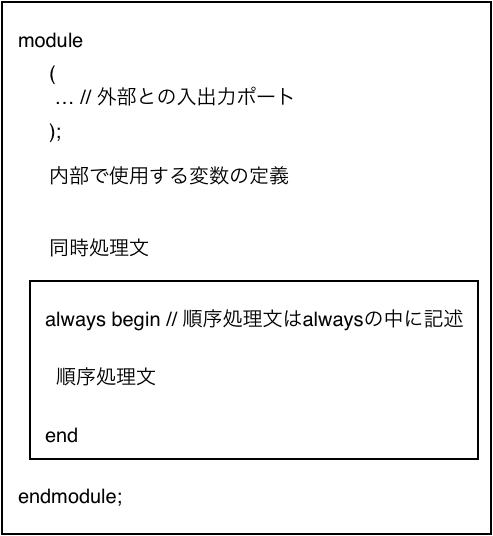
\includegraphics[width=.4\textwidth]{chapter02_figures/verilog_module_overview.png}
  \end{center}
  \caption{Verilog HDLのモジュール定義の概要 \label{fig:verilog_module_overview}}
 \end{figure}

\subsection{値の表現方法}
Verilog HDLでは,必要とするビット幅(\verb|w|)と基数(\verb|f|)を付けて「\verb|w'f値|」という形式で即値を記述します.ビット幅は10進数で記述します.ビット幅と基数を省略すると10進数,32bitの値になります.表\ref{tbl:verilog_value}に,基数と記号と表現される数の関係を示します.

\begin{table}[H]
\begin{center}
 \begin{tabular}{l|l|l|l}
 \hline
  基数(w) & 基数記号(f) & 例            & 10進数表記での値 \\\hline\hline
  2       & \verb|b|    & \verb|8'b10|  & 2 \\\hline
  10      & \verb|d|    & \verb|10'd10| & 10 \\\hline
          &             & \verb|10|     & 10 \\\hline
  16      & \verb|h|    & \verb|8'h10|  & 16 \\\hline
 \end{tabular}
\end{center}
\caption{Verilog HDLにおける値の表記例\label{tbl:verilog_value}}
\end{table}

\subsection{型 --- ネット型変数とレジスタ変数}
Verilog HDLの変数には,ネット変数とレジスタ変数があります.どちらも1bitの信号に相当する変数と,複数bitの信号を束にした配列変数を作れます.ネット変数とレジスタ変数の違いは,ハードウェアに則したワイヤ(配線)とレジスタ(記憶素子)を想起させるものですが,後で説明するように使える場面と使い方に違いがあります.表\ref{tbl:verilog_types}に,変数の型を示します.

\begin{table}[H]
\begin{center}
 \begin{tabular}{l|l}
 \hline
  型名               & 説明 \\\hline\hline
  \verb|wire|        & 1-bitのネット変数 \\\hline
  \verb|wire[n-1:0]| & n-bitのネット変数 \\\hline
  \verb|reg|         & n-bitのレジスタ変数 \\\hline
  \verb|reg[n-1:0]|  & n-bitのレジスタ変数 \\\hline
 \end{tabular}
\end{center}
\caption{Verilog HDLにおける型の例\label{tbl:verilog_types}}
\end{table}

\subsubsection{ネット変数 --- wire}
モジュールやゲート同士を接続する配線に名前を付けた変数が,ネット変数\verb|wire|です.ネット変数自身は値を保持することはできず,他から代入された値を次に伝達する役目を担う変数です.ハードウェアの配線そのものに相当します.

\subsubsection{レジスタ変数 --- reg}
レジスタ変数\verb|reg|は,値を保存する記憶素子になることができ,変数自身が値を保持できます.組み合わせ回路も順序回路も構成できます.

\subsubsection{配列変数}
配列変数\verb|wire[n-1:0]|,\verb|reg[n-1:0]|は,それぞれ\verb|wire|あるいは\verb|reg|からなるn-bitの変数に相当します.幅\verb|n|のネット変数
\begin{figure}[H]
\begin{quote}
\begin{Verbatim}[frame=single, numbers=left, baselinestretch=0.8]
wire[n-1:0] a;
reg[n-1:0] b;
\end{Verbatim}
\end{quote}
\end{figure}
と定義された変数aの各要素をa[0],a[2:0]などとして取り出すことができます.前者はwire,後者はwire[2:0]の変数です.

\subsection{モジュールの外枠の記述 --- module}
Verilog HDLでは,\verb|module|でハードウェア・モジュールの外枠を定義します.モジュールの名前と入出力の信号名を定義します.
\begin{figure}[H]
\begin{quote}
\begin{Verbatim}[frame=single, numbers=left, baselinestretch=0.8]
module test(pClk, pReset, Q);
\end{Verbatim}
\end{quote}
\end{figure}
この文では,\verb|pClk|,\verb|pReset|,\verb|Q|という名前の入出力信号を持つ\verb|test|という名前のモジュールを定義しています.
Verilog HDLでは,この\verb|module|文から
\begin{figure}[H]
\begin{quote}
\begin{Verbatim}[frame=single, numbers=left, baselinestretch=0.8]
endmodule
\end{Verbatim}
\end{quote}
\end{figure}
というキーワードまでがモジュールの定義に相当します.
moduleの末尾には‘;’(セミコロン)が必要ですが,endmoduleには付けないことに注意してください.
ポート名だけを列挙する場合には,後で,各ポートの入出力方向と幅を定義する必要があります.

少し前のVerilog-95
\begin{figure}[H]
\begin{quote}
\begin{Verbatim}[frame=single, numbers=left, baselinestretch=0.8]
module test(pClk, pReset, Q);
\end{Verbatim}
\end{quote}
\end{figure}


\subsubsection{ポートの定義}
ポートとは,モジュールの入出力信号のことです.ポートの名前は,モジュール名に続く()の中に記述します.
それぞれのポートの入出力は,モジュールの中で,「方向 型 変数名;」で宣言します.
方向には,\verb|input|(入力)と\verb|output|(出力),\verb|inout|(入出力)の3種類があります.
\verb|module|文の\verb|()|内に与えた信号線の型と入出力方向はモジュールの内部で定義します.
たとえば,\verb|pClk|と\verb|pReset|が1bitの入力,\verb|Q|が1bitの出力信号であれば,
\begin{figure}[H]
\begin{quote}
\begin{Verbatim}[frame=single, numbers=left, baselinestretch=0.8]
module test(pClk, pReset, Q);
  input   wire pClk;
  input   wire pReset;
  output  wire Q;

  // 以降,モジュールの内部処理を記述する

endmodule
\end{Verbatim}
\end{quote}
\end{figure}
と記述されます.

通常Verilog HDLでは,1bitのwire変数は定義せずに使えるため,wireが省略されることがあります.
もちろん,n-bitのポートを定義することもでます.Qが幅n-bitの出力ポートであれば,
\begin{figure}[H]
\begin{quote}
\begin{Verbatim}[frame=single, numbers=left, baselinestretch=0.8]
output wire[n-1:0] Q
\end{Verbatim}
\end{quote}
\end{figure}
と書けます.

Verilog-2001以降をサポートする処理系の場合には,VHDLのように信号名の定義に型と変数を付けることができます.
\begin{figure}[H]
\begin{quote}
\begin{Verbatim}[frame=single, numbers=left, baselinestretch=0.8]
module test(
  input wire pClk, 
  input wire pReset,
  output wire Q
);

  // 以降,モジュールの内部処理を記述する

endmodule
\end{Verbatim}
\end{quote}
\end{figure}
と記述できます.

\subsubsection{定数を定義する}
module宣言の後に,各モジュール内で有効な定数をparameter文で定義できます.
\begin{figure}[H]
\begin{quote}
\begin{Verbatim}[frame=single, numbers=left, baselinestretch=0.8]
module test(pClk, pReset, Q);
parameter width  = 640;
parameter height = 480;
\end{Verbatim}
\end{quote}
\end{figure}
上記に示したモジュールtestの中では,widthを640という値として利用できます.

\subsection{内部処理の記述}
ポートの宣言に引き続いて,内部で使用する変数の宣言および処理本体を記述します.

\subsection{変数の定義}
処理に必要な変数をあらかじめ定義しておく必要があります.変数は,ネット接続型あるいはレジスタ型の型を伴って定義されます.
\begin{figure}[H]
\begin{quote}
\begin{Verbatim}[frame=single, numbers=left, baselinestretch=0.8]
wire a;
reg[15:0] b;
\end{Verbatim}
\end{quote}
\end{figure}
これは,ネット変数\verb|a|と幅16ビットのレジスタ変数\verb|b|を定義しています.

また,\verb|parameter|で定義した定数\verb|width|を用いて,次のように変数を定義することもできます.
\begin{figure}[H]
\begin{quote}
\begin{Verbatim}[frame=single, numbers=left, baselinestretch=0.8]
reg[width-1:0] c;
\end{Verbatim}
\end{quote}
\end{figure}

\subsection{演算子と演算}
代表的な演算子を表\ref{tbl:verilog_operator}にまとめました.
論理演算における真と偽は,ネット変数やレジスタ変数の場合は\verb|'1'|と\verb|'0'|に対応します.
n-bitの配列変数\verb|wire[n-1:0]|あるいは\verb|reg[n-1:0]|の場合には,配列中に一つでも\verb|'1'|である要素があれば真,さもなければ偽として判定されます.ビット論理演算子を配列変数に適用する場合は,対応する各要素同士について演算が適用されます.

\begin{table}[H]
\begin{center}
 \begin{tabular}{l|l|l}
 \hline
  種類           & 演算子           & 説明 \\\hline\hline
  論理演算       & \verb|a && b|    & 論理積.aとbが共に真なら真.さもなければ偽.\\\cline{2-3}
                 & \verb|a || b|    & 論理和.aとbのどちらか又は両方が真なら真.さもなければ偽.\\\cline{2-3}
                 & \verb|!a|        & 否定.aが真なら偽.偽なら真\\\hline
  ビット論理演算 & \verb|a & b|     & 論理積.aとbが共に'1'なら'1'.さもなければ'0'.\\\cline{2-3}
                 & \verb|a | b|     & 論理和.aとbのどちらか又は両方が'1'なら'1'.さもなければ'0'.\\\cline{2-3}
                 & \verb|a ^ b|     & 排他的論理和.aとbのどちらか一方が'1'なら'1'.さもなければ'0'.\\\cline{2-3}
                 & \verb|~a|        & 論理否定.aが'1'なら'0'.さもなければ'1'.\\\hline
  比較演算       & \verb|a == b|    & aとbが等しい場合\verb|true|.さもなければ\verb|false|\\\cline{2-3}
                 & \verb|a != b|    & aとbが等しくなければ場合\verb|true|.さもなければ\verb|false|\\\cline{2-3}
                 & \verb|a > b|     & aがbがより大きいなら\verb|true|.さもなければ\verb|false|.(*1)\\\cline{2-3}
                 & \verb|a < b|     & aとbがより小さいなら\verb|true|.さもなければ\verb|false|.(*1)\\\cline{2-3}
                 & \verb|a >= b|    & aとb以上なら\verb|true|.さもなければ\verb|false|.(*1)\\\cline{2-3}
                 & \verb|a <= b|    & aとb以下なら\verb|true|.さもなければ\verb|false|.(*1)\\\hline
  算術演算       & \verb|a + b|     & aとbの足し算\\\cline{2-3}
                 & \verb|a - b|     & aとbの引き算\\\cline{2-3}
                 & \verb|a * b|     & aとbの引き算\\\cline{2-3}
                 & \verb|a / b|     & aとbの割り算\\\cline{2-3}
                 & \verb|a % b|     & aとbの割り算の余り\\\hline
   シフト演算    & \verb|a >> b|    & aとbビット,右にシフト \\\cline{2-3}
                 & \verb|a << b|    & aをbビット,左にシフト \\\hline
   条件演算      & \verb|a ? b : c| & aが真の時b,偽のときc \\\hline
   配列操作      & \verb|{a,b,c}|   & aとbとcをこの順に並べた信号線の束を作る \\\cline{2-3}
                 & \verb|a[b] |     & aのb番目の信号を取り出す \\\cline{2-3}
                 & \verb|a[b:c]|    & aのb番目からc番目の信号線の束を取り出す \\\hline
 \end{tabular}
\end{center}
\caption{Verilog HDLで用いられる演算の例\label{tbl:verilog_operator}}
\end{table}

\subsubsection{演算結果の代入}
演算の結果をネット変数あるいはレジスタ変数に代入できます.
ネット型変数への代入には\verb|assign|命令を使用して,下記のように記述します.
\begin{figure}[H]
\begin{quote}
\begin{Verbatim}[frame=single, numbers=left, baselinestretch=0.8]
assign c = a & b;
\end{Verbatim}
\end{quote}
\end{figure}
これは,ハードウェア的には,演算の結果を信号線に接続することに相当します.
ネット変数の代入は後述の同時処理文としてしか記述できません.

一方,レジスタ変数への代入では,ブロッキング代入とノンブロッキング代入の両方が使えます.
Verilog HDLでは,それぞれ下記のように記述します.
\begin{figure}[H]
\begin{quote}
\begin{Verbatim}[frame=single, numbers=left, baselinestretch=0.8]
=  // ブロッキング代入
<= // ノンブロッキング代入
\end{Verbatim}
\end{quote}
\end{figure}
たとえば,\verb|a + b|の演算結果をノンブロッキング代入する場合には,
\begin{figure}[H]
\begin{quote}
\begin{Verbatim}[frame=single, numbers=left, baselinestretch=0.8]
c <= a + b;
\end{Verbatim}
\end{quote}
\end{figure}
のように記述します.
レジスタ変数への値の代入は,ブロッキング代入とノンブロッキング代入のどちらも,
後で説明する順次処理文内でのみ使えます.

\subsubsection{型の変換}
VHDLが型に対して厳格であるのに対して,Verilog HDLでは暗黙のうちに型が変換されます.
意識せずに異なるビット幅の変数を演算,代入できます.

\subsubsection{シフト演算}
VHDLと異なり,Verilog HDLにはシフト演算子がありますが,シフト演算は大きな回路になってしまいます.
定数分のシフトを行いたい場合は,配列の結合演算を用いて実装する方が小さな回路として実現できます.
たとえば,配列変数reg[n-1:0]のcounterを右に1bitシフトしたい場合は,下記のようになります.
\begin{figure}[H]
\begin{quote}
\begin{Verbatim}[frame=single, numbers=left, baselinestretch=0.8]
{1'b0, counter[n-1:1]};
\end{Verbatim}
\end{quote}
\end{figure}
また,左に2つシフトしたい場合には,
\begin{figure}[H]
\begin{quote}
\begin{Verbatim}[frame=single, numbers=left, baselinestretch=0.8]
{counter[n-3:0], 2'b00};
\end{Verbatim}
\end{quote}
\end{figure}
のように記述します.

\subsection{同時処理文}
ネット型変数の演算結果の代入は,同時処理文を記述します.
記述されたすべての同時処理文は,合成ツールにより同時に解析され,回路として合成されます.
つまり,記述された内容は,その順序に依存しません.たとえば,
\begin{figure}[H]
\begin{quote}
\begin{Verbatim}[frame=single, numbers=left, baselinestretch=0.8]
assign c = a & b;
assign e = c & d;
\end{Verbatim}
\end{quote}
\end{figure}
という同時処理文の列も,
\begin{figure}[H]
\begin{quote}
\begin{Verbatim}[frame=single, numbers=left, baselinestretch=0.8]
assign e = c & d;
assign c = a & b;
\end{Verbatim}
\end{quote}
\end{figure}
の列も,同じように図8の回路が合成されます.

\subsection{順次処理文〜always文}
\verb|always|文は,順次処理文を記述するためのブロックを作るものです.順次処理文では,記述された順序に従って意味が解析され,
回路が合成されます.そのため,複雑な制御構文を使用できます.
基本的な構文を下記に示します.変数\verb|c|,\verb|d|は\verb|reg|変数です.
\begin{figure}[H]
\begin{quote}
\begin{Verbatim}[frame=single, numbers=left, baselinestretch=0.8]
always @(a, b) begin
  c <= a & b;
  d <= a | b;
end
\end{Verbatim}
\end{quote}
\end{figure}

ここで,\verb|always @()|の「\verb|()|」内の変数のリストをセンシティビティ・リストといいます.
このリストに列挙した変数が変化すると,プロセス文の中の回路の値が変更されます.
ノンブロッキング代入は,always内の処理の解釈がすべて完了したタイミングで,同時更新されることに注意してください.
このalways文は,図\ref{fig:process_example}のような回路になります.

\verb|always|文の中にある入力変数(式の右辺にでてくる変数)がすべてセンシティビティ・リストに列挙されている場合,
入力が変化する度に回路が動作し,出力変数(式の左辺)の値が変更されます.
つまり,その\verb|always|文は,何も状態を保存する必要がありません.
そのため,記憶素子を必要としない組み合わせ回路として構成されます.
ここで,入力に対して常に出力が生成されない場合とは,条件分岐などによって,
入力信号の値によって値の代入が発生しない出力信号がある場合です.

次のような\verb|always|文を考えてみます.
\begin{figure}[H]
\begin{quote}
\begin{Verbatim}[frame=single, numbers=left, baselinestretch=0.8]
always @(a) begin
  c <= a & b;
  d <= a | b;
end
\end{Verbatim}
\end{quote}
\end{figure}
ここでは,センシティビティ・リストに「\verb|b|」がなく,入力変数が全部列挙されていません.
この回路では,bの値が変化しても出力先であるcとdの値は変化しません.
つまり,図\ref{fig:process_example}のように,入力であるaとbを出力のcとdに直接接続することができず,
\verb|c|と\verb|d|の値を保存する機構,記憶素子が必要となり,組み合わせ回路としては合成されません.
「同じように記述したつもりでも違う回路になるかもしれない」ということを覚えておいてください.

\verb|always|の中では,\verb|reg|変数にブロッキング代入することもできます.
ブロッキング代入では,\verb|always|中のほかの代入に関係なく,その時点で代入が発生し値が置き換わります.
たとえば,次のような\verb|always|文を考えます.ここで,\verb|tmp0|,\verb|tmp1|,\verb|c|はすべて\verb|reg|変数とします.
\begin{figure}[H]
\begin{quote}
\begin{Verbatim}[frame=single, numbers=left, baselinestretch=0.8]
always @(a,b) begin
  tmp0 = a & b;
  tmp1 = a | b;
  c <= tmp0 ^ tmp1;
end
\end{Verbatim}
\end{quote}
\end{figure}
この場合,\verb|tmp0|と\verb|tmp1|ともに,ブロッキング代入で演算の結果が代入されています.
ブロッキング代入なので,合成ツールがこの構文に出会ったところで,\verb|tmp0|は\verb|(a & b)|に,
\verb|tmp1|は\verb|(a \| b)|にすぐさま置き換わます.つまり,これは単に\verb|c <= (a & b) ^ (a \| b)|という回路に合成されます.

センシティビティ・リストには,\verb|@(a and b)|という条件式が記述できます.
これはaとbのどちらかが変化した場合ではなく,\verb|(a and b)|が変化した場合に\verb|always|の中の処理を実行できるようにします.
条件式には,信号の立ち上がり,あるいは立ち下がり条件を使用することもできます.
立ち上がりは「posedge」,立ち下がりは「negedge」というキーワードを使います.
\begin{figure}[H]
\begin{quote}
\begin{Verbatim}[frame=single, numbers=left, baselinestretch=0.8]
alwasy @(posedge clk) begin
  処理文
end
\end{Verbatim}
\end{quote}
\end{figure}
これは,「clkの立ち上がり」のときに処理文が実行されることを意味します.
ハードウェア的には,clk信号が立ち上がった瞬間に相当し,それ意外のタイミングでは,処理文は動作せず,値が保存し続けられます.
これは,決まったタイミングで処理を実行する順序同期回路の設計に欠かせない表現です.

\subsection{制御構文}
ソフトウェア・プログミングのように,条件分岐のifやCでいう\verb|switch|構文のような制御構文が使えます.
多くの制御構文は,\verb|always|文の中でのみ使用することができます.代表的なものを次に説明します.

\subsubsection{if 〜 begin 〜 end else begin 〜 end --- 条件分岐構文}
\verb|always|文の中でのみ使用できる条件分岐構文です.
次に示す例では,\verb|a|が\verb|b|より大きければ処理文\verb|X|が,それ以外の場合は処理文\verb|Y|が実行されます.
また,処理文の中で,ifをネスト(入れ子)にすることもできます.
\begin{figure}[H]
\begin{quote}
\begin{Verbatim}[frame=single, numbers=left, baselinestretch=0.8]
if (a > b) begin
  処理文X
end else begin
  処理文Y
end
\end{Verbatim}
\end{quote}
\end{figure}

\subsubsection{case --- 選択}
CやJavaでいうところのswitch構文です.
次に示す例では,変数\verb|a|の値によって処理文X,Y,Zに分岐しています.
\verb|case|構文では,どれかのケースに該当するように記述しましょう.
もちろん,すべての条件を列挙してもよいのですが,「\verb|default|」でどんな値にもマッチする場合を記述できます.
\begin{figure}[H]
\begin{quote}
\begin{Verbatim}[frame=single, numbers=left, baselinestretch=0.8]
case(a)
  0 :
    処理文X
  1 :
    処理文Y
  2 :
    処理文Z
  default :
    処理文W
endcase
\end{Verbatim}
\end{quote}
\end{figure}

\subsubsection{繰り返し構文 for}
Verilog HDLにおける繰り返し処理は,単に似たような処理を繰り返して記述する代わりに簡単に書けるようにするための構文です.
実際には,繰り返し回数分のハードウェア回路が生成されます.
たとえば,下記に示す処理ですが,
\begin{figure}[H]
\begin{quote}
\begin{Verbatim}[frame=single, numbers=left, baselinestretch=0.8]
tmp = 1'b0;
for (i = 0; i < 5; i = i + 1) begin
  tmp = tmp | a[i];
end
b <= tmp;
\end{Verbatim}
\end{quote}
\end{figure}
これは,次のような代入文を記述することに相当します.
\begin{figure}[H]
\begin{quote}
\begin{Verbatim}[frame=single, numbers=left, baselinestretch=0.8]
tmp = 1'b0;
tmp = tmp | a[0];
tmp = tmp | a[1];
tmp = tmp | a[2];
tmp = tmp | a[3];
tmp = tmp | a[4];
b <= tmp;
\end{Verbatim}
\end{quote}
\end{figure}

\subsection{組み合わせ回路のサブモジュール}
Verilog HDLでは,複雑な組み合わせ回路を生成するために,\verb|function|というサブモジュールを記述できます.
\verb|function|は順次処理文で,\verb|if|や\verb|case|などの条件文を記述できますが,
ノンブロッキング代入を用いることはできません.\verb|function|は,次のように定義します.
\begin{figure}[H]
\begin{quote}
\begin{Verbatim}[frame=single, numbers=left, baselinestretch=0.8]
function f;
  input a;
  input b;
  begin
    if(a == b) begin
      f = 1'b1;
    end else begin
      f = 1'b0;
    end
  end
endfunction
\end{Verbatim}
\end{quote}
\end{figure}
これは,1ビットのネット型信号である\verb|a|と\verb|b|を入力とする名前\verb|f|の\verb|function|の定義です.
\verb|function|の中で\verb|f|に値を代入すると,関数の返り値としてセットされます.
この例は,入力された二つの値が等しいときに'1'を,異なるときに'0'を出力する関数です.

呼び出し側では,
\begin{figure}[H]
\begin{quote}
\begin{Verbatim}[frame=single, numbers=left, baselinestretch=0.8]
assign x = f(x, y)
\end{Verbatim}
\end{quote}
\end{figure}
または,always文で
\begin{figure}[H]
\begin{quote}
\begin{Verbatim}[frame=single, numbers=left, baselinestretch=0.8]
x <= f(x, y)
\end{Verbatim}
\end{quote}
\end{figure}
などとして呼び出せます.ここで,xとyは,関数呼び出しに対する実引数になります.

また,次のように,配列型の変数を入力あるいは出力する関数を定義できます.
\begin{figure}[H]
\begin{quote}
\begin{Verbatim}[frame=single, numbers=left, baselinestretch=0.8]
function [1:0] g; 
  input [1:0] x;
  begin
    g[0] = x[1];
    g[1] = x[0];
  end
endfunction
\end{Verbatim}
\end{quote}
\end{figure}
ここで定義した\verb|function|は,Cの関数とは違い,関数の計算が終了するまで呼び出し側の処理が待たされるような制御を伴うことはなく,
複雑な組み合わせ回路を見通し良く記述するための書き方です.

\section{まとめ}
ハードウェア記述言語であるVHDLとVerilog HDLの基本について説明しました.
どちらも一般のソフトウェア・プログラミング言語ではなじみの薄い,
\begin{itemize}
 \item ノンブロッキング代入とブロッキング代入
 \item 同時処理文や順次処理文
\end{itemize}
といった,ハードウェアを設計するための特有の特徴をもっています.
とはいえ,分岐構文などを使うと,ハードウェアで実装したい処理をソフトウェア的に設計できます.

今回は,基本的な文法の説明をかけあしで紹介しました.
ソフトウェア・プログラミングを習得する際にはある程度,文法を覚えたあとは,
他人の書いたコードをたくさん読むことで,言語をスムーズに習得できます.
ハードウェアを設計するためのHDLプログラミングでも同じです.
たとえば,OpenCores.orgには,さまざまなHDLコードが投稿されており,
また,米国Sun Microsystems社からは,SPARCプロセッサのHDLコードが公開されています.
習うより慣れろで,どんどん読み書きしてみましょう.

\section*{参考文献}
\begin{enumerate}
 \item Douglas L.Perry(著),メンター・グラフィックス・ジャパン株式会社(翻訳);VHDL(Ascii software science—Language),1996年10月,アスキー.
 \item Bhasker(著),デザインウェーブ企画室(翻訳);VHDL言語入門—ハードウェア記述言語によるロジック設計マスタリング(C\&E TUTORIAL),1995年7月,CQ出版社.
 \item 長谷川 裕恭;VHDLによるハードウェア設計入門—言語入力によるロジック回路設計手法を身につけよう,2004年4月,CQ出版社.
 \item 小林 優;入門Verilog HDL記述—ハードウェア記述言語の速習\&実践 改訂,2004年5月,CQ出版社.
 \item 井倉 将実;FPGAボードで学ぶVerilog HDL,2007年2月,CQ出版社.
\end{enumerate}

\end{document}
